The theoretical congestion threshold $d_{i}^{*}$ is not satisfactory as it monitors "noisy" congestion (situations of free-flow that is at the limit of the congestion), distorting $E_{CP}$ results. We add a small number of vehicles $\delta$ (in our case, $\delta=6$) to this threshold in order to monitor only the hardcore congestion that our congested domain $\widetilde{\mathscr{C}}$ is supposed to capture.
	\begin{equation*} 
		d_{i}^{*}=\frac{Link\ capacity}{Link\ freeflow\ speed}+\delta
	\end{equation*}
As we are trying to fit an average congestion, we define the data congested domain $\widetilde{\mathscr{C}}$ as a set of boxes that roughly capture each congestion structure.\\
The average data density contour plot and the unique box we defined in our case are displayed below :
\begin{figure}[h!]
	\centering
	\caption{Density contour plot on the average data from 5 Tuesdays. Dark blue vertical strips are un-monitored mainline links.}
	\label{fig:pems_contour}
	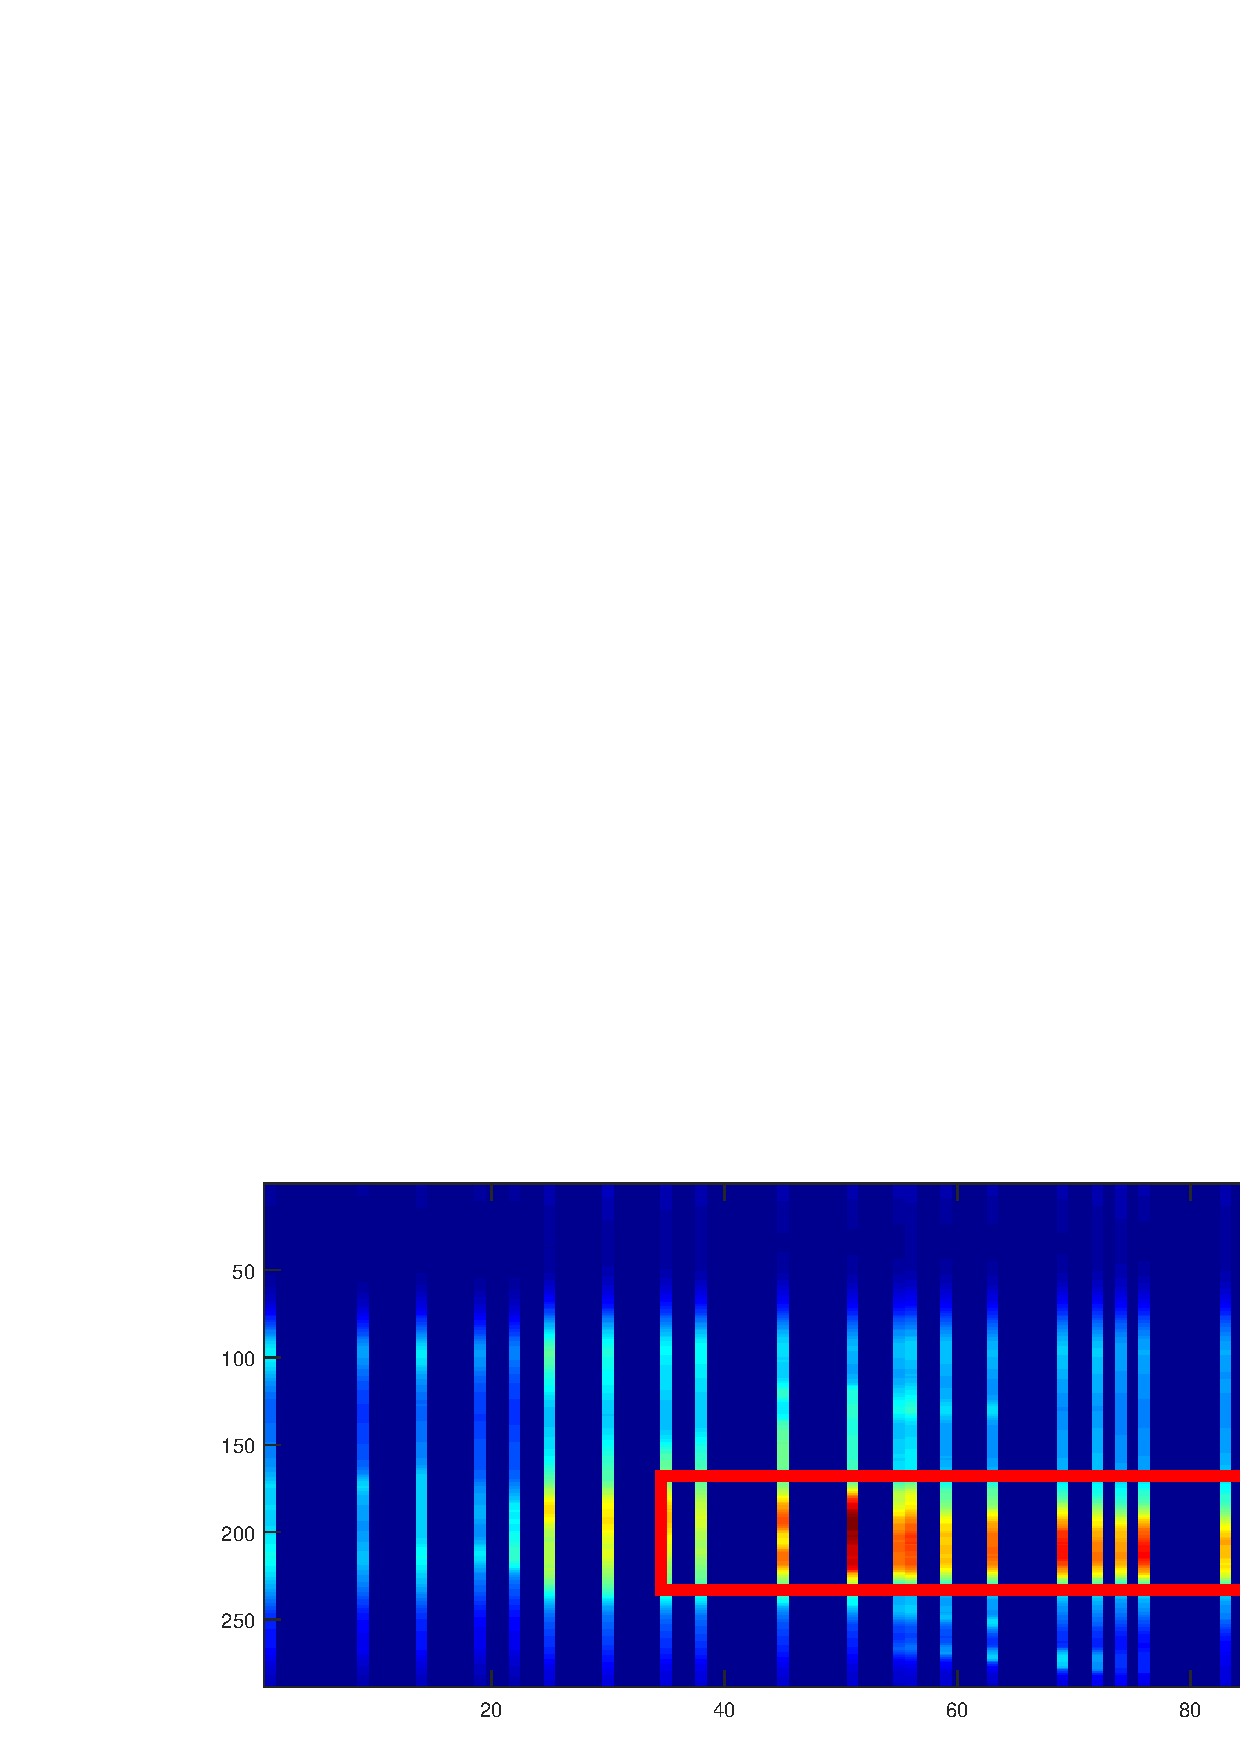
\includegraphics[width=7in]{figures/PeMS_contour.png}
\end{figure}
